\documentclass{jarticle}

\setlength{\voffset}{-65pt}
\setlength{\oddsidemargin}{-5mm}
\setlength{\textwidth}{490pt}
\setlength{\textheight}{700pt}

\usepackage{graphicx}
\usepackage{amsmath,amssymb,pifont,colortbl,amscd, wrapfig, ascmac}
\usepackage{amsthm}
\usepackage{url}
\usepackage{bm}
\newtheorem{theorem}{定理}
\newtheorem{definition}{定義}
\newtheorem{example}{例}

\def\ev{\mathrm{ev}}
\def\c{\mathop{\mathrm{cts}}\nolimits}
\def\odd{\mathop{\mathrm{odd}}\nolimits}
\def\diag{\mathop{\mathrm{diag}}\nolimits}
\def\mod{\mathop{\mathrm{mod}}\nolimits}
\def\deg{\mathop{\mathrm{deg}}\nolimits}
\def\inv{\mathop{\mathrm{Inv}}\nolimits}
\def\cl{\mathop{\mathrm{cl}}\nolimits}
\def\ad{\mathop{\mathrm{ad}}\nolimits}
\newcommand{\sad}{\overline{\ad}}
\def\tr{\mathop{\mathrm{tr}}\nolimits}
\def\End{\mathop{\mathrm{End}}\nolimits}
\def\id{\mathop{\mathrm{id}}\nolimits}
\def\ev{\mathop{\mathrm{ev}}\nolimits}
\def\coev{\mathop{\mathrm{coev}}\nolimits}
\def\coad{\mathop{\mathrm{coad}}\nolimits}
\def\Ob{\mathop{\mathrm{Ob}}\nolimits}
\def\Hom{\mathop{\mathrm{Hom}}\nolimits}
\def\im{\mathop{\mathrm{Im}}\nolimits}
\def\Span{\mathop{\mathrm{Span}}\nolimits}
\def\ideal{\mathop{\mathrm{ideal}}\nolimits}
\def\co{\colon\thinspace}
%for U_h
\newcommand{\uqenh}[1]{ (\bar U_q^{\ev})\,\hat  {}^{\;\hat  \otimes #1}}
\newcommand{\uqen}[1]{ (\bar U_q^{\ev})\;\tilde {}^{\;\tilde \otimes #1}}
\newcommand{\uqe}{\bar U_q^{\ev}}
\newcommand{\uqz}{\bar U_q^0}
\newcommand{\uqze}{\bar U_q^{\ev 0}}
\newcommand{\uq}{\bar U_q}
\newcommand{\muq}{\mathcal{ U}_q}
\newcommand{\muqe}{\mathcal{ U}_q^{\ev}}
\newcommand{\uqzq}{U_{\mathbb{Z},q}}
\newcommand{\uqzqe}{(U_{\mathbb{Z},q})^{\ev}}
\newcommand{\uqn}[1]{\bar U_q^{\otimes {#1}}}
\newcommand{\uhn}[1]{\bar U_h^{\hat \otimes {#1}}}
\newcommand{\f}[1]{\tilde F^{({#1})}}
\newcommand{\e}[1]{\tilde E^{({#1})}}
\newcommand{\Z}{\mathbb{Z}[q,q^{-1}]}
\def\ZA{\mathbb{P}^{\mathrm{fin}}\big( \Hom_{\mathcal{A}}(0,g)\big)}

\def\deg{\mathop{\mathrm{deg}}\nolimits}
\def\inv{\mathop{\mathrm{Inv}}\nolimits}
\def\cl{\mathop{\mathrm{cl}}\nolimits}
\def\ad{\mathop{\mathrm{ad}}\nolimits}
\def\tr{\mathop{\mathrm{tr}}\nolimits}
\def\End{\mathop{\mathrm{End}}\nolimits}
\def\id{\mathop{\mathrm{id}}\nolimits}
\def\ev{\mathop{\mathrm{ev}}\nolimits}
\def\coev{\mathop{\mathrm{coev}}\nolimits}
\def\coad{\mathop{\mathrm{coad}}\nolimits}
\def\Ob{\mathop{\mathrm{Ob}}\nolimits}
\def\Hom{\mathop{\mathrm{Hom}}\nolimits}
\def\Sets{\mathop{\mathrm{Sets}}\nolimits}
\def\im{\mathop{\mathrm{Im}}\nolimits}
\def\co{\colon\thinspace}

%%% ywr extend 
\def\d{\mathrm d}
\def\grad{\mathrm grad}
\def\rot{\mathrm{\bm rot}}
\def\div{\mathrm{div}}
%%%

\begin{document}

\title{微分積分続論(ベクトル解析)} 
\author{鈴木 咲衣}
\date{平成27年度前期}
\maketitle

\begin{center} {\Large 演習問題8 } \end{center}
\begin{enumerate}
\item \cite[練習問題4.9, 4.11, 章末問題4.5]{koba} 次の領域の面積を面積分により計算せよ.
\begin{enumerate}
\item 点$(0,0,1), (2,0,1),(2,1,1), (0,1,1)$を頂点とする長方形.
\item 原点を中心とする半径$3$の球面の$z>0$の部分.
\item $z$軸を中心とし,半径$3$の円筒の側面の$-1\leq z\leq 2$の部分.
\item 平行四辺形$\psi(s,t)=(s,t,2s+3t)$, $0\leq s\leq 1, 0\leq t\leq 1$.
\item 回転放物面$\psi(t, \theta)=(t\cos \theta,t\sin \theta, t^{2})$, $0\leq \theta \leq 2\pi, 0\leq t\leq 1$.
\item $xy$平面上の楕円$x^{2}+\frac{y^{2}}{4}=1$の内部の面積.
\end{enumerate}
\item \cite[章末問題4.6]{koba} 次の$S$と$f$の組に対して面積分$\int_{S}f dS$を計算せよ.
\begin{enumerate}
\item $S$は点$(0,0,3), (2,0,3),(2,1,3), (0,1,3)$を頂点とする長方形. $f=xyz$.
\item $S=\psi(s,t)=(s,t,st)$, $0\leq s\leq 1, 0\leq t\leq 1$. $f=xy$.
\item  $S=\psi(t,\theta)=(1+t\cos \theta ,1+t\sin \theta, t)$, $0\leq t\leq 1, 0\leq \theta \leq \pi$. $f=x+z^{2}$.
\end{enumerate}
\item  \cite[章末問題4.7]{koba} パラメータ$s,t$で表された曲面$(s\cos t, s\sin t, s)$の$0\leq s \leq 1$, $0\leq t\leq 2\pi$の部分を$S$とする.
\begin{enumerate}
\item $S$の概形を描け.
\item $S$の面積を求めよ.
\end{enumerate}
\end{enumerate}

\newpage

\begin{center} {\Large 演習問題8 解答} \end{center}
\begin{enumerate}
  \item
    \begin{enumerate}
      \item
        \[ \int_0^2 \d x \int_0^1 \d y = 2 \]
      \item
        求めるべき領域を$D$とおくと,
        \[ \int_D r^2 \sin \theta \d \theta \d \phi = 9 \int_0^{\frac{\pi}{2}} \sin \theta \d \theta \int_0^{2\pi} \d \phi = 9 \cdot 1 \cdot 2 \pi = 18 \pi \]
      \item
        求めるべき領域を$D$とおくと,
        \[ \int_D r \d \theta \d z = r \int_{-1}^2 \d z \int_0^{2\pi} \d \theta = 3 \cdot 3 \cdot 2 \pi = 18 \pi \]
      \item
        $|(1,0,2) \times (0,1,3)| = |(-2,-3,1)| = \sqrt{14}$より,
        \[ \sqrt{14} \int_0^1 \int_0^1 \d s \d t = \sqrt{14} \]
      \item
      
        \begin{eqnarray*}
        \left|\frac{\partial \psi}{\partial s} \times \frac{\partial \psi}{\partial t} \right| & = & \left|  (-t\sin\theta,t\cos\theta, 0) \times  (\cos\theta,\sin\theta,2t) \right| \\
        & = & \left| (2t^2\cos\theta, 2t^2\sin\theta,-t) \right| \\
        & = & t\sqrt{4t^{2}+1 }
        \end{eqnarray*}
        よって求めるべき面積$S$は,
        \[ S = \int_0^1  t\sqrt{4t^{2}+1 } \d t \int_0^{2\pi} \d \theta = \frac{1}{12}(5\sqrt{5}-1)\cdot 2\pi = \frac{\pi}{6} (5\sqrt{5}-1) \]
      \item
        楕円は$x=r\cos\theta,y=2r\sin\theta$ただし$0 \leq r \leq 1, 0 \leq \theta < 2\pi$と表示できる.
        \[ 
          \left| \begin{array}{cc}
            \cos\theta & -r\sin\theta \\
            2\sin\theta & 2r\cos\theta
          \end{array} \right| = 2r
        \]
        よって求めるべき面積$S$は,
        \[
          S = \int_0^1 2r \d r \int_0^{2\pi} = 1 \cdot 2\pi = 2\pi
        \]
    \end{enumerate}
  \item

       
    \begin{enumerate}
      \item
        \[ \int_S f \d S = 3 \int_0^2 x \d x \int_0^1 y \d y = 3 \cdot \frac{4}{2} \cdot \frac{1}{2} = 3 \]
      \item
        \[ | (1,0,y) \times (0,1,x) | = | (-y,-x,1) | = \sqrt{1+x^2+y^2} \]
        より,
        \begin{eqnarray*} 
          \int_0^1 \d x \int_0^1 \d y xy \sqrt{1+x^2+y^2} & = & \int_0^1 \d x \left[ \frac{1}{3} x (1+x^2+y^2)^\frac{3}{2} \right]_0^1 \\
          & = & \int_0^1 \d x \frac{1}{3} x \left\{ (2+x^2)^{\frac{3}{2}} - (1+x^2)^{\frac{3}{2}} \right\} \\
          & = & \frac{1}{3} \left[ \frac{1}{5} (2+x^2)^\frac{5}{2} - \frac{1}{5} (1+x^2)^\frac{5}{2} \right]_0^1 \\
          & = & \frac{1}{3} \left( \frac{1}{5} 3^\frac{5}{2} - \frac{1}{5} 2^\frac{5}{2} - \frac{1}{5} 2^\frac{5}{2} + \frac{1}{5} \right) \\
          & = & \frac{1}{15} \left( 3^\frac{5}{2} - 2^\frac{7}{2} + 1 \right)\\
          & = & \frac{1}{15} \left( 9 \sqrt{3}- 8\sqrt{2} + 1 \right)
        \end{eqnarray*}
      \item  \begin{eqnarray*}
        \left|\frac{\partial \psi}{\partial t} \times \frac{\partial \psi}{\partial \theta} \right| & = & \left|  (\cos\theta,\sin\theta, 1) \times  (-t\sin\theta,t\cos\theta,t) \right| \\
        & = & \sqrt{2}t
         \end{eqnarray*}
         より
           \begin{eqnarray*} 
          \int_0^1 \int _{0}^{\pi} \left( (1+t \cos \theta+ t^{2}) \sqrt{2} t \d \theta \d t \right) 
          & = &\sqrt{2} \int_{0}^{1} t [\theta +t\sin \theta +t^{2} \theta]_{0}^{\pi} \d t \\
          & = & \sqrt{2} \int_{0}^{1} t (\pi +\pi t^{2}) \d t \\
          & = & \sqrt{2} \pi \left[\frac{t^{2}}{2}+ \frac{1}{4} t^{4}\right]_{0}^{1} \\
          & = & \frac{3}{4} \sqrt{2} \pi
                  \end{eqnarray*}
      
    \end{enumerate}
  \item   
       
    \begin{enumerate}
      \item 
      \begin{picture}(10,50)
\put(0,-150){ 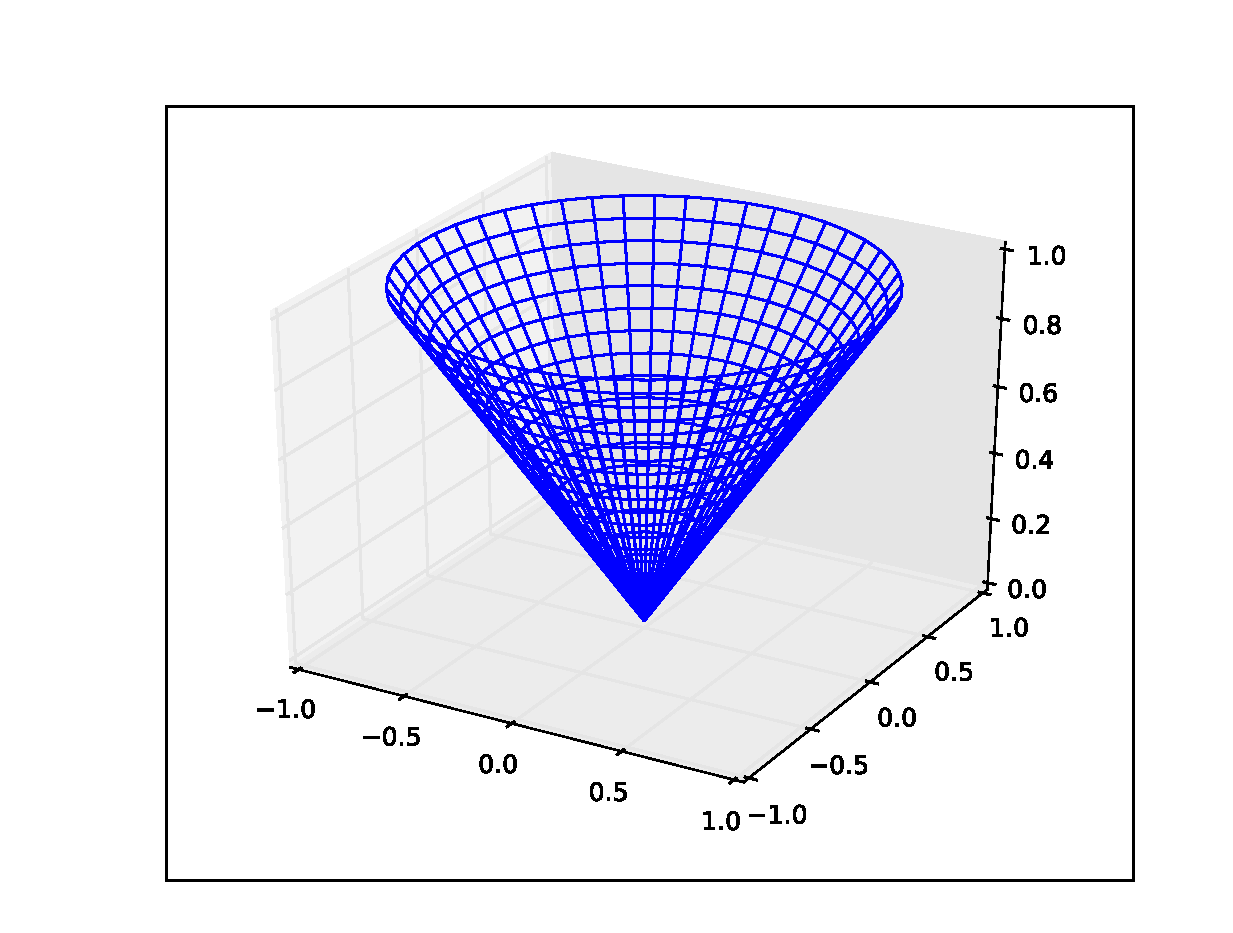
\includegraphics[width=9cm,clip]{answer_8_3_a.eps}}
\end{picture}
     
     \vspace{150pt}
        
          %\begin{figure}
          %  \begin{center}
          %    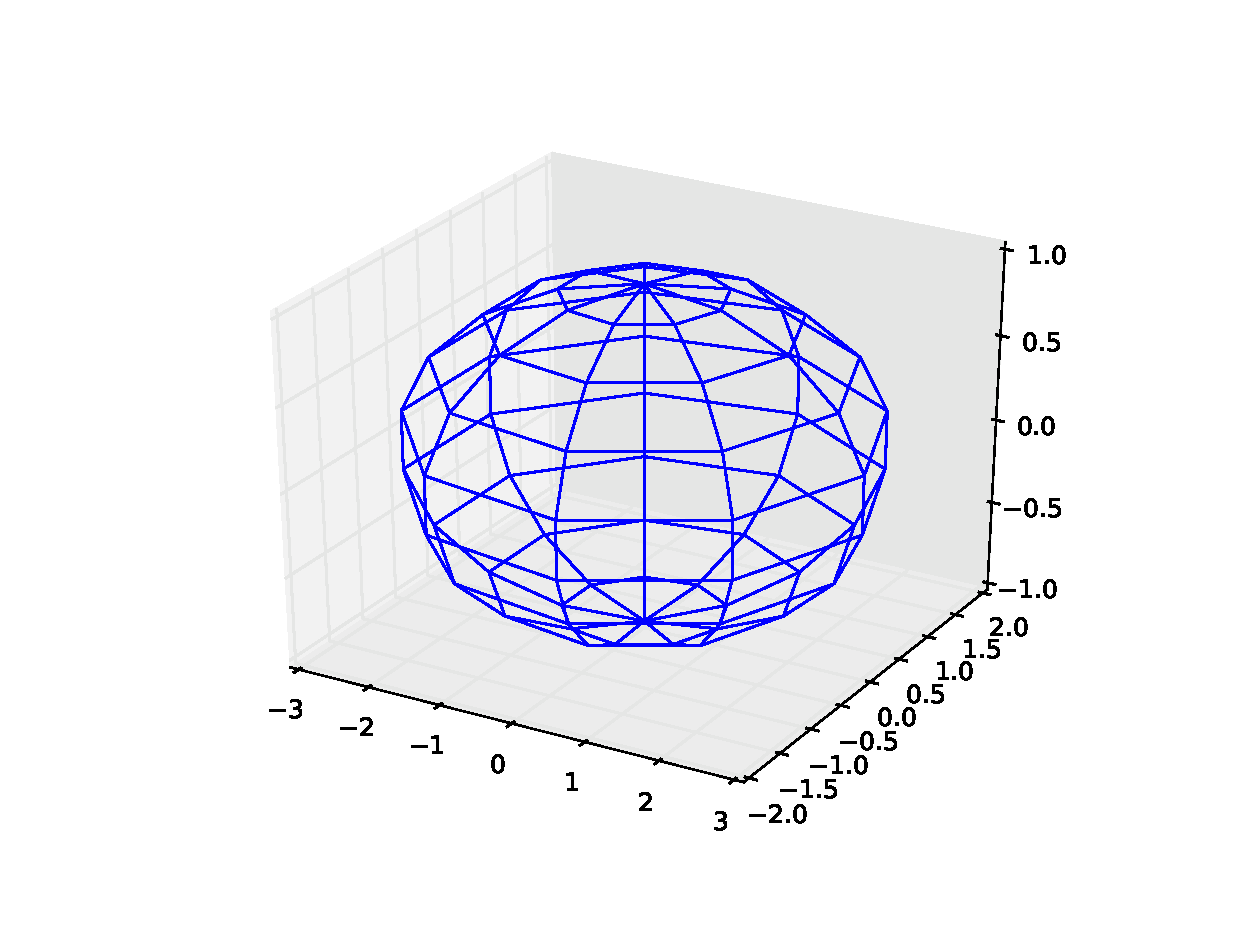
\includegraphics[height=6cm]{answer_9_1_a.eps}
          %  \end{center}
          %\end{figure}
      \item
        \[ (\cos t,\sin t,0) \times (-s\sin t,s\cos t,1) = s(\sin t,-\cos t, 1) \]
        よって,
        \[ \int_S \d S = \sqrt{2} \int_0^1 s \d s \int_0^{2\pi} \d t = \sqrt{2} \cdot \frac{1}{2} \cdot 2\pi = \sqrt{2} \pi\]
    \end{enumerate}
\end{enumerate}
  \newpage
\begin{thebibliography}{99}
\bibitem[2]{koba} 小林亮,高橋大輔「ベクトル解析入門」(東京大学出版会)

\end{thebibliography}

\end{document}